\section{Introduction}

This document is my research internship report, whose initial subject matter was to model the temporal dependencies between recurring patterns in electrophysiology, namely in data obtained by capturing electrical and magnetic activity of the brain.
However, this report will focus on modelling the temporal dependency between external stimuli and recurring patterns.
The general method is derived from Hawkes processes, a specific type of temporal point processes, but with a different approach that we called \textit{driven temporal point processes}.

First, we will rapidly describe the working environment of Inria and more specifically the Parietal team.
Then, the general problematic of the work presented in this report will be detailed.
Will follow some background on both data in electrophysiology and on signals decomposition via dictionary learning.
Finally, a presentation of the theory of point processes will be done, with a focus on temporal point processes, as it is the theoretical tool used in this work.

\subsection{Inria and Parietal team}

I did my internship at Inria Saclay, within the Parietal team, under the supervision of \href{http://alexandre.gramfort.net}{Alexandre Gramfort}, senior research scientist, and \href{https://tommoral.github.io/about.html}{Thomas Moreau}, research scientist, both permanent members of the Parietal team.
This section aims to briefly present the research institute of Inria, with a focus on the Parietal team.

\paragraph{Inria} The \href{https://www.inria.fr/fr}{Institute for Research in Computer Science and Automatic} (Inria\footnote{Institut de recherche en informatique et en automatique}) is a national institute for research in digital science and technology.
It has been funded in 1967, within the framework of the ``\textit{Plan Calcul}''\footnote{The Plan Calcul was a French governmental program launched in 1966 by President Charles de Gaulle designed to ensure the country's autonomy in information technology, and to develop European IT.}, and employs \num{3500} researchers and engineers often working in an interdisciplinary manner and in collaboration with industrial partners.
Inria Saclay is one of the 9 research centres spread over the territory that compose Inria.
 Also, thanks to \href{https://learninglab.inria.fr}{Inria Learning Lab}, Inria designs MOOCs to disseminate knowledge in digital sciences and strengthen the dialogue between science and society.


\paragraph{Parietal team} Within Inria, reasearchers are divided among \num{200} project-teams, the \href{https://team.inria.fr/parietal/}{Parietal team} being one of them.
It is an Inria-CEA joint team part of the Neurospin research center, headed by \href{https://pages.saclay.inria.fr/bertrand.thirion/}{Bertrand Thirion}, that focuses on mathematical methods for statistical modeling of brain function using neuroimaging data (fMRI, MEG, EEG), with a particular interest in machine learning techniques, applications to human cognitive neuroscience, and scientific software development\footnote{Source: presentation of Parietal, \url{https://team.inria.fr/parietal/}}.
The different members of Parietal are committers to a variety of open-source projects such as Scikit-Learn, 
NiLearn and MNE-Python, among others.

\subsection{General problematic}

As previously mentioned, the data that are mainly used by the person working in the Parietal team come from electroencephalography (EEG) and magnetoencephalography (MEG), two methods used to record neuronal activity of the brain.
The M/EEG data we are interested in for the following of the report are acquired during experiments with human subjects, that consist in a recording of the neuronal activity for a duration around 3 to 7 minutes.
In the following Section~\ref{data_in_electrophysiology}, more info will be given on how the brain neuronal activity is produced and recorded

During the experiment, different type of external stimuli can be exercised on the subject, such as an auditory signal (left or right side, at different frequencies), a visual signal (left and right eye), the action to press a button, etc.
The term external stimuli is opposed to an internal stimuli, where the subject would be ask to think at something or to think at doing something, without really doing it.
In Section~\ref{res_real_data}, the data and the different types of stimuli will be presented in more detail.

The main objective of this report is to model the temporal dependency between a specific stimulus and its neuronal response.
To do so, we decompose the signal into recurring patterns, called \textit{atoms}, using to dictionary learning and convolutional sparse coding, as it will be presented in Section~\ref{meeg_decomposition}.
More specifically, we would like to model the latency between external stimuli and neuronal responses, or, in other words, model how a given stimulus can `activate' a specific atom in the brain, and thus, find the atom(s) that have a high probability to be linked with a specific external stimulus.

To respond to such a problematic, a new method will be introduced in Section~\ref{developed_method}, and it is based on temporal point process, more particularly on Hawkes processes.
We called this new method \textit{driven temporal point process}.
Before presenting our method, a background on point processes with a focus on temporal point processes will  be done  in Section~\ref{background_tpp}.

%TODO:  what for? a possible practical application?
 
\subsection{Data in electrophysiology (M/EEG)}\label{data_in_electrophysiology}

Electrophysiology refers to a branch of physiology that study the electrical and electrochemical phenomena that occur in the cells or tissues of living organisms and, in particular, in neurons and muscle fibres.
In neuroscience, we are particularly interested in the electrical activity of the neurons and especially in the emission of post-synaptic potentials (PSP).
In a neuron, PSP are nerve influx along the axon consecutive to ion exchange at the synapse level, as shown in Figure~\ref{fig:post_synaptic_potentials}, which change the polarity of the cell membrane.
As moving charges on a wire induces an electo-magnetic field, a group of neurons in the gray matter\footnote{More precisely, the pyramidal cells in the cortex, that constitute approximately \SI{80}{\percent} of the neurons of the cortex.}, the upper part of the brain that is composed essentially of the cell bodies and the dendritic tree of neurons, form a current generator\footnote{Alexandre \textsc{Gramfort}, \textit{ Functional Brain Imaging with MEG, EEG and sEEG}, Université Paris-Saclay, MEEG course, \url{http://bit.ly/meeg_course}} that produces an electrical and a magnetic field.

\begin{figure}[h]
    \centering
    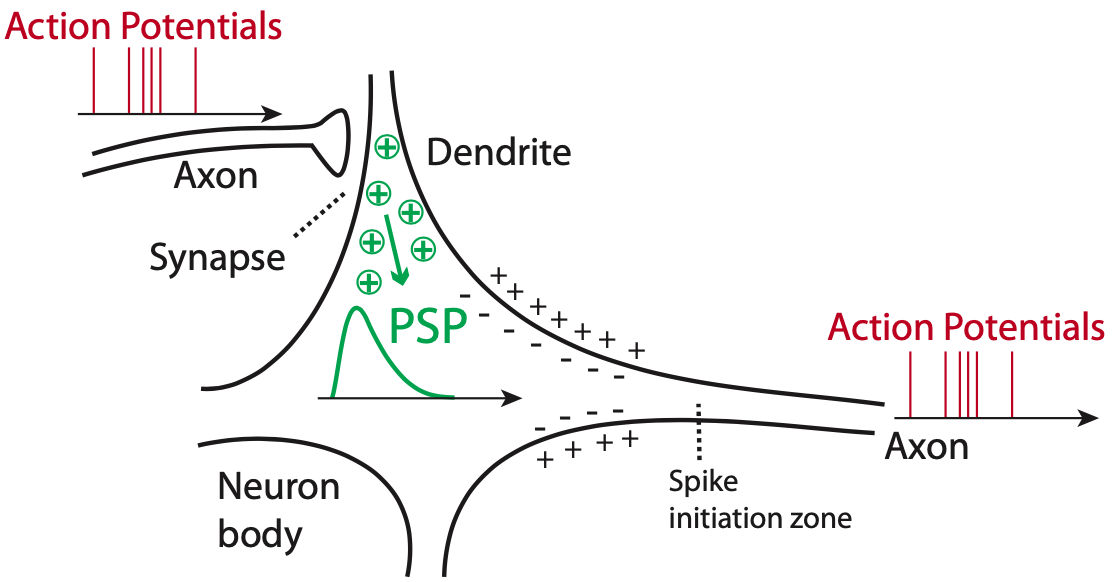
\includegraphics[scale=0.25]{pics/post-synaptic_potentials.png}
    \caption{Post-synaptic potentials in a neuron, consecutive to ion exchange}
    \source{A. \textsc{Gramfort}, MEEG course}
    \label{fig:post_synaptic_potentials}
\end{figure}

Two methods are used to capture both the electrical and the magnetic field, respectively the electroencephalography (EEG) that captures differences in electric potential at the scalp, and the magnetoencephalography (MEG) that captures magnetic flux density outside the head, as shown in Figure~\ref{fig:meeg_recordings}.
Both method record synchronised neural activity at a very high temporal resolution, about the millisecond\footnote{Sampling is often between \num{250} and \SI{1000}{\hertz}.}, and have the advantage of being non-invasive, unlike ectrocorticography (ECoG) that uses electrodes placed directly on the exposed surface of the brain.
Note that a large number of simultaneously active neurons, about \num{50000}, are needed to generate a measurable M/EEG signal\footnote{Saskia \textsc{Helbling}, \textit{What are we measuring with M/EEG?}, Goethe University Frankfurt, SPM course, May 2014}.

\begin{figure}
    \centering
    \begin{subfigure}[h]{0.45\textwidth}
        \centering
        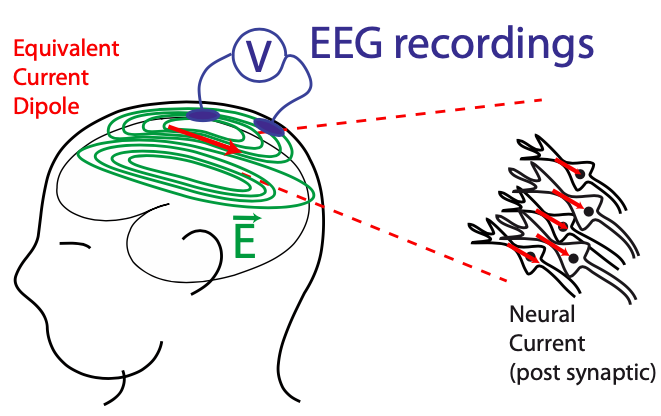
\includegraphics[width=0.9\textwidth]{pics/eeg_recordings.png}
        \caption{EEG recordings}
        \label{fig:eeg_recordings}
    \end{subfigure}
    \hfill
    \begin{subfigure}[h]{0.45\textwidth}
        \centering
        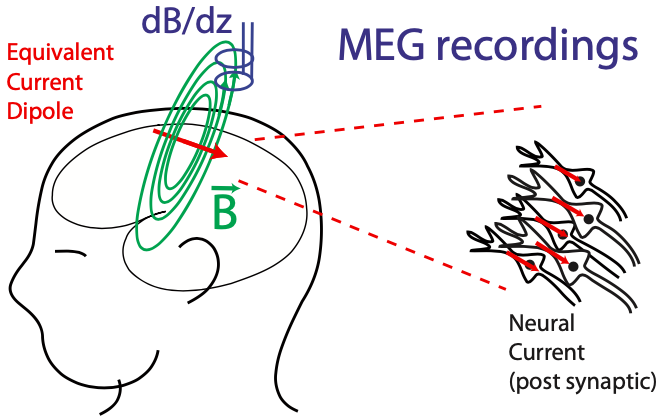
\includegraphics[width=0.9\textwidth]{pics/meg_recordings.png}
        \caption{MEG recordings}
        \label{fig:meg_recordings}
    \end{subfigure}
    \caption{Recordings of the electrical field (a) and the magnetic field (b).}
    \source{A. \textsc{Gramfort}, MEEG course}
    \label{fig:meeg_recordings}
\end{figure}

This high temporal resolution is what makes MEG and EEG attractive for the functional study of the brain.
The spatial resolution, on the contrary, is rather poor as only a few hundred simultaneous data positions can be acquired simultaneously (about \numrange{300}{400} sensors for MEG and up to \num{256} electrodes for EEG).
With appropriate models and methods, localisation of activity from MEG and EEG is nevertheless possible\footnote{\href{https://team.inria.fr/athena/fr/megeeg-vs-other-functional-brain-imaging-modalities/}{Inria: MEG/EEG vs. other functional brain imaging modalities}}.
This is what is called the \textit{inverse problem}, whose objective is to determine the current generators that produced the M/EEG measurements, as opposed to the \textit{forward problem} whose objective is to predict the M/EEG surface signal to current dipoles in the brain.

Finaly, note that neural activity recorded via M/EEG measurements is fundamental to modern experimental neuroscience and in our understanding of human cognitive processes and certain pathologies, thereby motivating the development of computational tools for learning such signals from data.
Such recordings consist of dozens to hundreds of simultaneously recorded signals, for duration going from minutes to hour \citep{jas2017learning, dupre2018multivariate}.

In this report we will mainly focus on the data recorded via MEG obtained in the course of experiments in which subjects are exposed to external stimuli.
A more comprehensive presentation of the data we work with is done in the Section~\ref{res_real_data}.
In Python, M/EEG data are easily manipulable thanks to the \href{https://mne.tools/stable/index.html}{\texttt{MNE} package} \citep{gramfort2013meg}.

\subsection{M/EEG signals decomposition via dictionary learning}\label{meeg_decomposition}

As previously explained in Section~\ref{data_in_electrophysiology}, the data recorded from one subject via M/EEG is complex.
For example, for $P$ sensors, called \textit{channels}, over $T$ timestamps, the signal observed is $X \in \R^{P\times T}$, that contains heavy noise bursts and have low signal-to-noise ratio, as most of neural signals \citep{jas2017learning}.
Thus, we cannot work directly with this result, we have to pre-process it in some way. 

It is known that neural time-series data contain a wide variety of prototypical signal waveforms (atoms) that are of significant importance in clinical and cognitive research.
One of the goals for analysing such data is hence to extract such `shift-invariant' atoms, as events can happen at any instant \citep{jas2017learning}.
While alpha waves (\SIrange{8}{12}{\hertz}) are known to closely resemble short sinusoids, and thus are revealed by Fourier analysis or wavelet transforms, there is an evolving debate that electromagnetic neural signals are composed of more complex waveforms that cannot be analysed by linear filters and traditional signal representations \cite{dupre2018multivariate}.

To learn such atoms, one method is to use \textit{dictionary learning}, that is a branch of signal processing and machine learning that aims at finding a frame (called dictionary) in which some training data admits a sparse representation.
The sparser the representation, the better the dictionary\footnote{\href{https://team.inria.fr/panama/fr/projects/please/dictionary-learning/}{Team Inria Panama - Dictionary learning: theory and algorithms}}.
Applied to brain signals, one method that works well is \textit{convolutional sparse coding} (CSC) \citep{jas2017learning, dupre2018multivariate, moreau2019distributed}.
This method aims at finding a dictionary of atoms and some associated activation vectors, in order to recover the original signal $X$ by doing a convolution between the atoms and their sparse activation vectors, as shown in Figure~\ref{fig:signal_decomposition}.

\begin{figure}[h!]
    \centering
    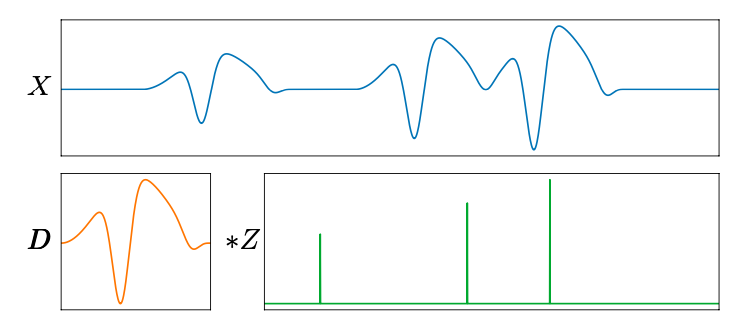
\includegraphics[scale=0.5]{pics/atom_decomposition.png}
    \caption{Decomposition of a noiseless univariate signal $X$ (blue) as the convolution $Z * \boldsymbol{D}$ between a temporal pattern $\boldsymbol{D}$ (orange) and a sparse activation signal $Z$ (green).}
    \source{\cite{moreau2019distributed}}
    \label{fig:signal_decomposition}
\end{figure}

The optimisation problem is as follow\footnote{Note that we are in the case of 1D-convolution, in multivariate CSC.}:
\begin{equation}\label{eq:csc_problem}
\begin{gathered}
\min _{D_{k}, z_{k}^{n}} \sum_{n=1}^{N} \frac{1}{2}\norme{X^{n}-\sum_{k=1}^{K} z_{k}^{n} * D_{k}}_{2}^{2}+\lambda \sum_{k=1}^{K}\norme{z_{k}^{n}}_{1} \\
\text { s.t. } \quad \norme{D_{k}}_{2}^{2} \leq 1 \text { and } z_{k}^{n} \geq 0
\end{gathered}
\end{equation}
where $\braces{X^n}_{n=1}^N \in \R^{P\times T}$ are $N$ observed multivariate signals, $\lambda > 0$ is the regularization parameter, $\braces{D_k}_{k=1}^K \in \R^{P\times L}$ are the spatio-temporal atoms, $\braces{z_k^n}_{k=1}^K \in \R^{\widetilde{T}}$ are $K$ sparse signals of activations associated with $X^n$, with $\widetilde{T} \coloneqq T - L + 1$, and where $z_{k}^{n} * D_{k}$ denotes the convolution between the two signals, obtained by by convolving every row of $D_k$ by $z_k^n$.

In order to better account for the nature of brain signals, a rank-1 constraint is added to the dictionary: $D_k = u_k v_k^T \in \R^{P\times L}$, with $u_k \in \R^P$ being the pattern over channels and $v_k \in \R^L$ over time.
Thus, the $\norme{D_{k}}_{2}^{2} \leq 1$ constraint in \eqref{eq:csc_problem} is now replaced by $\norme{u_{k}}_{2}^{2} \leq 1$ and $\norme{v_{k}}_{2}^{2} \leq 1$.
This rank-1 constraint comes from Maxwell's equations and the physical model of electrophysiological signals like EEG or MEG, where each sensor is supposed to instantly receive a linear transformation of every sources, with a constant topographic map, i.e., a signal coming from the same source at two different times will be spread across the sensors with the same linear transformation.
Thanks to this rank-1 constraint, the learned atoms have a spacial and a temporal pattern, as shown in Figure~\ref{fig:atom_location_and_form}.

\begin{figure}[h!]
    \centering
    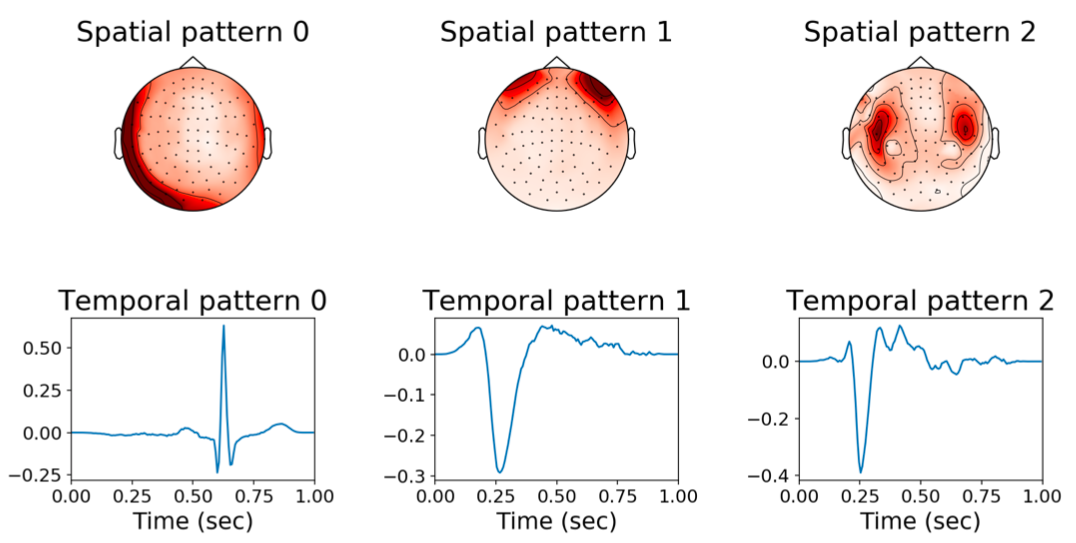
\includegraphics[scale=0.35]{pics/atom_location_and_form.png}
    \caption{Spacial (up) and temporal (down) representation of three atoms obtained by dictionary learning}
    %\source{\protect\href{https://alphacsc.github.io/auto_examples/multicsc/plot_sample_evoked_response.html#sphx-glr-auto-examples-multicsc-plot-sample-evoked-response-py}{Example in \texttt{alphacsc} package's documentation}}
    \source{Example in \texttt{alphacsc} package's documentation}
    \label{fig:atom_location_and_form}
\end{figure}

In python, the package \href{https://alphacsc.github.io/index.html}{\texttt{alphacsc}} makes it possible to carry out such an operation.
In practice, we do not have $N$ signals, as the brain of every person is different, it would make no sense to consider that the atoms of one subject are strictly identical to another.
Thus, we split the recorded signal $X\in\R^{P\times T}$ into several smaller signals, in order to take advantage of the factorised computations describe in \citep{dupre2018multivariate} that speed up computational time, and eventually to be able to distribute computations \citep{moreau2019distributed}\footnote{Note that distributed CSC is not implemented yet into \texttt{alphacsc}.}.
Once the original signal is split into $N$ smaller signals, the dictionary of atoms $D$ and their associated activations vectors $z_k^n$ are learned.
Finally, an ultimate action is done: with the learned dictionary $D$ and with the original signal $X$, the matrix $z \in \R^{K\times \widetilde{T}}$ is learned solving \eqref{eq:csc_problem}.

%\citep{jas2017learning}:
%\begin{itemize}
    %\item Neural time-series data contain a wide variety of prototypical signal waveforms (atoms) that are of significant importance in clinical and cognitive research. One of the goals for analyzing such data is hence to extract such ‘shift-invariant’ atoms.
    
    %\item convolutional sparse coding (CSC) model for learning shift-invariant atoms from raw neural signals containing potentially severe artifacts.
    
    %\item A natural way to cast the problem of learning a dictionary of shift-invariant atoms into an optimization problem is a convolutional sparse coding (CSC) approach
    
    %\item As opposed to using generic bases that have predefined shapes, such as the Fourier or the wavelet bases, these atoms provide a more meaningful representation of the data and are not restricted to narrow frequency bands.
    
    %\item neural signals often contain heavy noise bursts and have low signal-to-noise ratio.
%\end{itemize}

%Résumé de \cite{dupre2018multivariate}:
%\begin{itemize}
    %\item Frequency-specific patterns of neural activity are traditionally interpreted as sustained rhythmic oscillations, and related to cognitive mechanisms such as attention, high level visual processing or motor control. While alpha waves (8–12 Hz) are known to closely resemble short sinusoids, and thus are revealed by Fourier analysis or wavelet transforms, there is an evolving debate that electromagnetic neural signals are composed of more complex waveforms that cannot be analyzed by linear filters and traditional signal representations.
    
    %\item In this paper, we propose to learn dedicated representations of such recordings using a multivariate convolutional sparse coding (CSC) algorithm. Applied to electroencephalography (EEG) or magnetoencephalography (MEG) data, this method is able to learn not only prototypical temporal waveforms, but also associated spatial patterns so their origin can be localized in the brain.
    
    %\item Dictionary learning is one family of techniques, which consists in learning atoms (or patterns) that offer sparse data approximations.
    
    %\item When working with long signals in which events can happen at any instant, one idea is to learn shift-invariant atoms. They can offer better signal approximations than generic bases such as Fourier or wavelets, since they are not limited to narrow frequency bands.
    
    %\item In this study, we develop a multivariate model for CSC, using a rank-1 constraint on the atoms to account for the instantaneous spreading of an electromagnetic source over all the channels. -> Maxwell equation, thanks to the rank-1 model can be localized in the brain for clinical or cognitive neuroscience studies.
    
    %\item bien expliquer l'hypothèse de rang 1, comme quoi c'est une conséquence de la linéarité et de l'immédiateté des équations de Maxwell. Pour un capteur $x_n$, le signal reçu peut être représenté comme étant $S$ (l'ensemble de tous les signaux) plus un signal $v_k$ (issu d'un dipole dans le cerveau, ici intervient l'immédiateté du signal, il n'y a pas de latence) multiplié par une constante $u_{n,k}$ (ici intervient la linéarité, tous les capteurs reçoivent en même temps le même signal magnétique, à une transformation linéaire près). Ainsi, puisque l'on peut faire de même avec tous les capteurs, on peut représenter les signaux reçu comme étant $X = S + u_k v_k^T$, et ainsi on trouve que $X = \sum_k u_k v_k^T$ (le tout multiplié par un $z_k$, qui lui détermine l'activation dans le temps)
%\end{itemize}
\subsection{Background on point processes}\label{background_tpp}

In this section, we will give a short introduction on point processes, and particularly on temporal point processes with a focus on Hawkes processes.
Further details can be found in \citep{daley2003introduction, daley2007introduction}.
The sub-section~\ref{pp_definitions} comes from the PhD thesis of Massil Achab~\citep{achab2017learning}.

\subsubsection{Definitions}\label{pp_definitions}
A point process is a random element whose values are point patterns on a set $S$, a locally compact metric space equipped with its Borel $\sigma$-algebra $\mathscr{B}$.
Let $X_S$ be the set of locally finite counting measures on $S$, and $\mathcal{N}_S$ the smallest $\sigma$-algebra on $X_S$ such that all point counts ${f_B: X_s \to \N, \omega \mapsto \#\pars{\omega \cap B}}$ are measurable for $B$ relatively compact in $\mathscr{B}$, where $\# A$ denotes the cardinality of the set $A$.
A point process on $S$ is a measurable map $\xi$ from a probability space $\pars{\Omega, \mathcal{F}, \proba{}}$ to the measurable space $\pars{X_S, \mathcal{N}_S}$.

Every realisation of a point process $\xi$ can be written as $\xi = \sum_{i=1}^n \dirac_{X_i}$, where $\dirac$ is the Dirac measure, $n$ is a integer-valued random variable and $X_i$'s are random elements of $S$.
A point process can be equivalently represented by a counting process $N\pars{B} \coloneqq \integ{B}{\xi (x)}{x}$ which basically is the number of event in each Borel subset $B\in\mathscr{B}$.
The mean measure $M$ of a point process $\xi$ is a measure on $S$ that assigns to every $B\in\mathscr{B}$ the expected number of event of $\xi$ in $B$, i.e., $M\pars{B} \coloneqq \esp{N\pars{B}}$ for all $B\in\mathscr{B}$.


\subsubsection{Temporal point processes}
A temporal point process is a stochastic, or random, process composed of a time series of binary events that occur in continuous time\footnote{\href{http://www.stat.columbia.edu/~liam/teaching/neurostat-fall19/uri-eden-point-process-notes.pdf}{Liam Paninski, Statistical analysis of neural data, Fall 2019, \textit{Chapter 2: Introduction to Point Processes} - Columbia Statistics}}.
However, on the contrary of time series, temporal point processes can study multiple time scales at once~\citep{bompaire2019machine}. 

In this particular case, $S$ is the time interval $\intervalleFO{0}{T}$, equipped with the Borel $\sigma$-field of the real line $\mathscr{B}\pars{\R}$.
Here, a realisation of a point process is simply a set of time points: $\xi = \sum_{i=1}^n \delta_{t_i}$.
With a slight abuse of notation, we associate to the set of distinct random timestamps $\xi = \braces{t_1, \dots, t_n}$ occurring before $T$, the counting process $N_t = \sum_{t_i \in\xi}\1[t_i \leq t]$, which is then simply the number of points in the time interval $\intervalleOF{0}{t}$.
This counting process is a random process which evolves over time by jumps of size 1.
Studying temporal point processes consists in analysing when this jumps occur.
The \textit{conditional intensity} function $\lambda\pars{t \middle| \mathscr{F}_t}$ is the usual way to characterise temporal point processes where the present depends on the past.
It is defined as the expected infinitesimal rate at which events are expected to occur after $t$ given the information $\mathscr{F}_t$ available up to (but not including) time $t$, i.e., the history of the counting process $N_t$ prior to $t$.
Namely,
\begin{equation}
    \lambda\pars{t \middle| \mathscr{F}_t} = \lim_{\dint t \to 0} \frac{\proba{N_{t + \dint t} - N_t = 1}[\mathscr{F}_t]}{\dint t}
\end{equation}
where $\mathscr{F}_t = \enstq{t_i}{t_i < t, i=1,\dots,n}$ is the natural filtration of the process.
The conditional intensity function is sometimes denoted $\lambda^*(t)$.

As $\dint N_t \coloneqq N_{t +\dint t} - N_t \in \braces{0,1}$ can only increase by one event at each $\dint t$, it readily follows that $\proba{\dint N_t = 1}[\mathscr{F}_t] = \lambda^*(t)\dint t$ and
\begin{equation}
    \esp{\dint N_t}[\mathscr{F}_t] = 1\times \proba{\dint N_t = 1}[\mathscr{F}_t] + 0\times \proba{\dint N_t = 0}[\mathscr{F}_t] = \lambda^*(t)\dint t
\end{equation}
Hence, we can also think of the conditional intensity function $\lambda^*(t)$ as an instantaneous rate of events per time of unit.

The \textit{homogeneous Poisson process} is the most simple temporal point process, which assumes that the events arrive at a constant rate, which corresponds to a constant intensity function $\lambda\pars{t \middle| \mathscr{F}_t} = \lambda^*(t) = \lambda > 0$.
In other words, it describe a phenomenon with no memory and a constant probability of occurrence in which $N_{t + \Delta t} - N_t$ follows a Poisson distribution of parameter $\Delta t$ for any $\Delta t > 0$.
For this process, $\forall B \in \mathscr{B}\pars{\R}, M\pars{B} = \lambda \abs{B}$, where $\abs{\cdot}$ is the Lebesgue measure on $\pars{S, \mathscr{B}\pars{\R}}$.

The \textit{inhomogeneous Poisson process} is a more general process, for which the conditional intensity function is not constant as it depends on $t$ but \textit{not} on the history, i.e. $\lambda\pars{t \middle| \mathscr{F}_t} = \lambda^*(t) = \lambda(t)$.
For this process, $M\pars{B} = \integ{B}{\lambda(x)}{x}$, for all $B \in \mathscr{B}\pars{\R}$.

Let us denote $f^*(t) = f\pars{t \middle| \mathscr{F}_t}$ the conditional probability density function of the inter-event time, i.e., the probability that the next event will occur during the interval $\intervalleFO{t}{t+\dint t}$ conditioned on the history $\mathscr{F}_t$.
Let us also denote $F^*(t) = F\pars{t \middle| \mathscr{F}_t} = \proba{t_n \leq t_{n+1} \leq t}[\mathscr{F}_t] =  \integ{t_{n}}[t]{f^*(\tau)}{\tau}$ the conditional cumulative density function, i.e., the probability that the next event will occur before time $t$ conditioned on the history $\mathscr{F}_t$, where here $t_n$ is the last event in $\mathscr{F}_t$, i.e., the last event before time $t$.
Finally, we denote $S^*(t) = 1 - F^*(t) = \proba{t_{n+1} \geq t}[\mathscr{F}_t]$ the complementary cumulative distribution, also called the survival function, i.e., the probability that the next event will not occur before time $t$ conditioned on the history $\mathscr{F}_t$ \citep{de2019temporal}.
Now,
\begin{equation}
    \begin{split}
        \lambda^*(t) &= \lim_{\dint t \to 0} \frac{\proba{t\leq t_{n+1} \leq t+\dint t}[t_{n+1} > t]}{\dint t} \\
        &= \lim_{\dint t \to 0} \frac{1}{\dint t} \frac{\proba{t\leq t_{n+1} \leq t+\dint t}}{\proba{t_{n+1} > t}} \\
        &= \lim_{\dint t \to 0} \pars{\frac{1}{\dint t}\frac{f^*(t)\dint t}{S^*(t)} + o(1)} \\
        &= \frac{f^*(t)}{S^*(t)} \\
        &= - \frac{1}{S^*(t)} \deriv{S^*(t)}{t} \\
        &= -\deriv{\log S^*(t)}{t}
    \end{split}
\end{equation}
By integrating the left and right hand sides in the above equation, we have that
\begin{equation}
    \integ{t_n}[t]{\lambda^*(\tau)}{\tau} = \integ{t_n}[t]{-\deriv{\log S^*(\tau)}{\tau}}{\tau} = -\log S^*(t) + \underbrace{\log S^*(t_n)}_{=0}
\end{equation}
and thus,
\begin{equation}
    S^*(t) = \e{- \integ{t_n}[t]{\lambda^*(\tau)}{\tau}}
\end{equation}
Finally, we get that
\begin{equation}\label{eq:f_star_res}
    f^*(t) = \lambda^*(t) \e{- \integ{t_n}[t]{\lambda^*(\tau)}{\tau}}
\end{equation}

\subsubsection{Poisson process and likelihood function}

This section is taken and adapted from \citep[chap.~2, p.~19-23]{daley2003introduction} and aims to give a more in-depth presentation of the Poisson processes, with a focus on the computation of the likelihood function, as it is a crucial information for the repport.

The stationary Poisson process\footnote{What we previously called the homogeneous Poisson process.}, on the line is completely defined by the following equation, in which we use $N\intervalleOF{a_i}{b_i}$ to denote the number of events of the process falling in the half-open interval $\intervalleOF{a_i}{b_i}$ with $a_i < b_i \leq a_i+1$:
\begin{equation}\label{eq:def_stationary_pp}
    \proba{N\intervalleOF{a_i}{b_i} = n_i, i=1,\dots,k} = \prod_{i=1}^k \frac{\bracks{\lambda\pars{b_i-a_i}}^{n_i}}{n_i!}e^{-\lambda\pars{b_i-a_i}}
\end{equation}

This definition embodies three important features:
\begin{itemize}
    \item the number of points in each finite interval $\intervalleOF{a_i}{b_i}$ has a Poisson distribution of parameter $\lambda$;
    
    \item the numbers of points in disjoint intervals are independent random variables; and
    
    \item the distributions are stationary: they depend only on the lengths $b_i - a_i$ of the intervals.
\end{itemize}

The likelihood of a finite realisation of a Poisson process may be defined as the probability of obtaining the given number of observations in the observation period, times the joint conditional density for the positions of those observations, given their number.

Suppose that there are $N$ observations on $\intervalleOF{0}{T}$ at time points $t_1,\dots,t_N$. From \ref{eq:def_stationary_pp}, we can write down immediately the probability of obtaining single events in $\intervalleOF{t_i-\Delta}{t_i}$ and no points on the remaining part of $\intervalleOF{0}{T}$.
Let $A$ and $B$ be respectively those events, namely, 
$$A = \braces{N\intervalleOF{t_i-\Delta}{t_i} = 1, i=1,\dots,N}$$
and
$$B = \braces{N\intervalleOF{0}{t_{1}-\Delta} = 0, N\intervalleOF{t_N}{T} = 0, N\intervalleOF{t_i}{t_{i+1}-\Delta} = 0, i=1,\dots,N-1}$$
\begin{align*}
    \proba{A\cap B} &= \prod_{i=1}^N \pars{\lambda\Delta e^{-\lambda\Delta}} \times e^{-\lambda\pars{t_1 - \Delta}} \times e^{-\lambda\pars{T-t_N}} \times \prod_{i=1}^{N-1} e^{-\lambda\pars{t_{i+1}-\Delta-t_i}} \\
    &= \prod_{i=1}^N \pars{\lambda\Delta} \times e^{-\lambda \Delta N} \times e^{-\lambda\pars{T-N\Delta}} \\
    &= e^{-\lambda T} \prod_{i=1}^N \lambda\Delta \\
    &= \lambda^N \Delta^N e^{-\lambda T}
\end{align*}

Dividing by $\Delta^N$ and letting $\Delta \xrightarrow{} 0$, to obtain the density, we find as the required likelihood function
\begin{equation}
    L_{\intervalleOF{0}{T}}\pars{N;t_1,\dots,t_n} = \lambda^N e^{-\lambda T}
\end{equation}

We can extend this result to a Poisson process with time-varying rate $\lambda(t)$, commonly called the \textit{nonhomogeneous} or \textit{inhomogeneous} Poisson process.
The process can be defined exactly as in \ref{eq:def_stationary_pp}, ,with the quantities $\lambda\intervalleOF{a_i}{b_i} = \integ{a_i}[b_i]{\lambda}{x}$ replaced wherever they occur by quantities
$$ \Lambda\intervalleOF{a_i}{b_i} = \integ{a_i}[b_i]{\lambda(x)}{x}$$
called the \textit{compensator} of the point process.
Thus, the joint distributions are still Poisson, and the independence property still holds.
The likelihood function takes the more general form
\begin{equation}\label{eq:general_likelihood}
\begin{split}
    L_{\intervalleOF{0}{T}}\pars{N;t_1,\dots,t_n} &= e^{-\Lambda\intervalleOF{0}{T}} \prod_{i=1}^N \lambda(t_i) \\
    &= \e{-\integ{0}[T]{\lambda(t)}{t} + \sum_{i=1}^N \log \lambda(t_i)} \\
    &= \e{-\integ{0}[T]{\lambda(t)}{t} + \int_0^T \log \lambda(t)N\pars{\dint t}}
\end{split}
\end{equation}

Note that this result could also be obtained by using the Equation~\eqref{eq:f_star_res}.

\subsubsection{Hawkes processes}\label{hawkes_processes}

In this section, we give the main definitions and properties of Hawkes processes and multivariate Hawkes processes and set the notations that will be used if the in the rest of the report.
Hawkes processes~\citep{hawkes1971point, hawkes1974cluster} are temporal point processes in which the intensity depends on the process history with an excitation mechanism.
They can be understood as the equivalent of auto-regressive time series models (AR) but in continuous time.
This allows to study cross causality that might occur in one or several events series~\citep{bompaire2019machine}.

An Hawkes process is thus defined by a history dependent intensity $\lambda$ defined as follows:
\begin{equation}\label{eq:uni_hawkes_process}
    \lambda\pars{t\middle| \mathscr{F}_t} = \psi\pars{\mu + \integ{-\infty}[t]{\phi(t-s)}{N_s}}
\end{equation}
where 
\begin{equation}
    \integ{-\infty}[t]{\phi(t-s)}{N_s} = \sum_{i, t_i<t} \phi(t-t_i)
\end{equation}
The $\mu \geq 0$ is referred as the \textit{baseline intensity}\footnote{Some authors may also call it the background intensity.} and it corresponds to the exogenous intensity of the considered events.
The function $\phi(\cdot):\R^+\to\R$ is called the \textit{kernel function}, or the transfer function~\citep{chen2017multivariate}, and quantifies over time and in magnitude the influence of past events.
Note that the occurrence of each event $t_i$ increases the intensity by a certain amount, determined by the kernel, making the intensity history dependent and a stochastic process by itself \citep{de2019temporal}.
If the \textit{link function} $\psi$ on the right-hand side of Eq.~\ref{eq:uni_hawkes_process} is non-linear, then $\lambda(t)$ is the intensity of a non-linear Hawkes process~\citep{bremaud1996stability}.
In what follows, we only consider the case where $\psi$ is the identity function.

\paragraph{Multivariate Hawkes process} We can extend the univariate Hawkes process to model the interactions of $K\geq 1$ temporal point processes, called \textit{nodes}.

Namely, it models timestamps $\braces{t_k^{(i)}}_{k\geq 1}$ of nodes $i=1,\dots,K$ associated with a multivariate counting process $N_t = \bracks{N_t^{(1)}, \dots, N_t^{(K)}}$.
Note that for all nodes $i=1,\dots,K$, we still have that all of its timestamps $t_k^{(i)}$ occur in the time interval $\intervalleFF{0}{T}$.
The excitation dynamic between the nodes is encompassed by the auto-regressive structure of the conditional intensity.
For component $N_t^{(i)}$ it writes
\begin{equation}
    \lambda_i\pars{t \middle| \mathscr{F}_t} = \mu_i + \sum_{j=1}^K  \integ{-\infty}[t]{\phi_{i,j}(t-s)}{N_s^{(j)}}
\end{equation}
where $\phi_{i,j}(t)$ quantifies the excitation rate of an event of type $j$ on the arrival rate of events of type $i$ after a time lag $t$.
In general it is assumed that each kernel is causal and positive, meaning that Hawkes processes can only account for mutual excitation effects since the occurrence of some event can only increase the future arrival intensity of other events.
If the kernels are integrable, each entry of the $K\times K$ matrix ${\pars{\Phi}_{i,j} = \integ{0}[T]{\phi_{i,j}(t)}{t}}$ denotes the expected number of events of type $i$ directly triggered by an event of type $j$.

\begin{figure}[h]
    \centering
    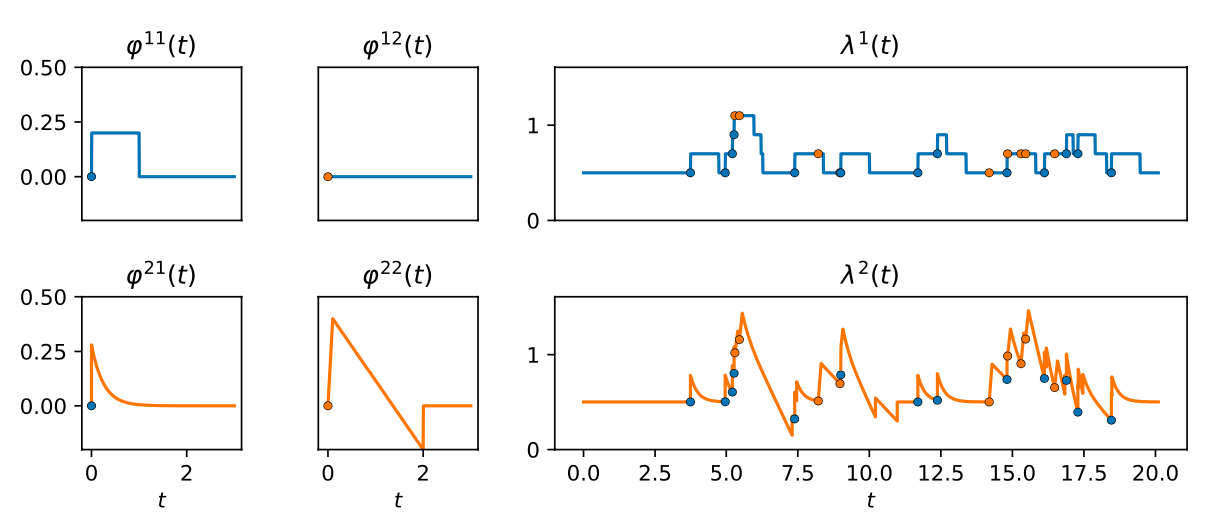
\includegraphics[scale=0.35]{pics/simu_multi_hawkes.png}
    \caption{A realisation of a 2 nodes multivariate Hawkes process. The four excitation kernels are shown on the left hand side. The intensities are displayed on the right hand side (against time, up to time 20), where events are represented by coloured dots (blue corresponding to node 1 and orange to node 2).}
    \source{\citep{bompaire2019machine}}
\end{figure}

\paragraph{Kernels parametrisation}
The main parametric model is the so-called \textit{exponential kernel}, in which the kernels have the following form:
\begin{equation}
    \phi_{i,j}(t) = \alpha_{i,j} \beta \e{-\beta t}, \quad \alpha_{i,j} > 0, \beta > 0
\end{equation}
In this model the integral matrix $\Phi = \pars{\alpha_{i,j}}_{1\leq i,j\leq K}$ and $\beta > 0$ is a memory parameter.
A more general approach is the \textit{sum of exponentials kernels}~\citep{lemonnier2014nonparametric}, namely
\begin{equation}
    \phi_{i,j}(t) = \sum_{u=1}^U \alpha_{i,j}^{(u)} \beta^{(u)} \e{-\beta^{(u)} t}, \quad \alpha_{i,j}^{(u)} > 0, \beta^{(u)} > 0
\end{equation}

Similarly, we can define the \textit{gaussian kernel} and the \textit{sum of gaussians kernels}.
In python, the \texttt{Tick} package allow to easily manipulate Hawkes process with exponential and gaussian kernels~\citep{bompaire2019machine, bacry2017tick}.
Other kernel functions are presented in~\citep{mehrdad2014hawkes}.
